\chapter{Implementation}

With the above described requirements, designs and specification, implementing the first MVP product started. The two teams were involved in the  development of product. One team focused on the development of ROS part required which is backend department. Other team focused on the frontend side of the project that is the UI/UX team. 

I was involved in the backend part of the team. My main goal was to create the services and topics to handling of the rosbag. Handling of the rosbag included like playing, pausing, jumping to the particular location of the rosbag, increasing the speed of the rosbag. With the previous research on the required library it was able to handle the rosbag with the rosservices. 

Some requirements of the project only was needed to be known by the frontend side. For example the duration of the rosbag. So those data are just published by the topic so that on the frontend side it can just be subscribed and get the data. 

Another major task was to create the REST-API for jobs which are not performed continuously and cannot be done only with rosservices. This included the upload of bag to cloud, updating of the map. This also included the downloading of bag from particular http link. The look of REST-API looks as shown in below figure
\begin{figure}[h]
	\begin{center}
		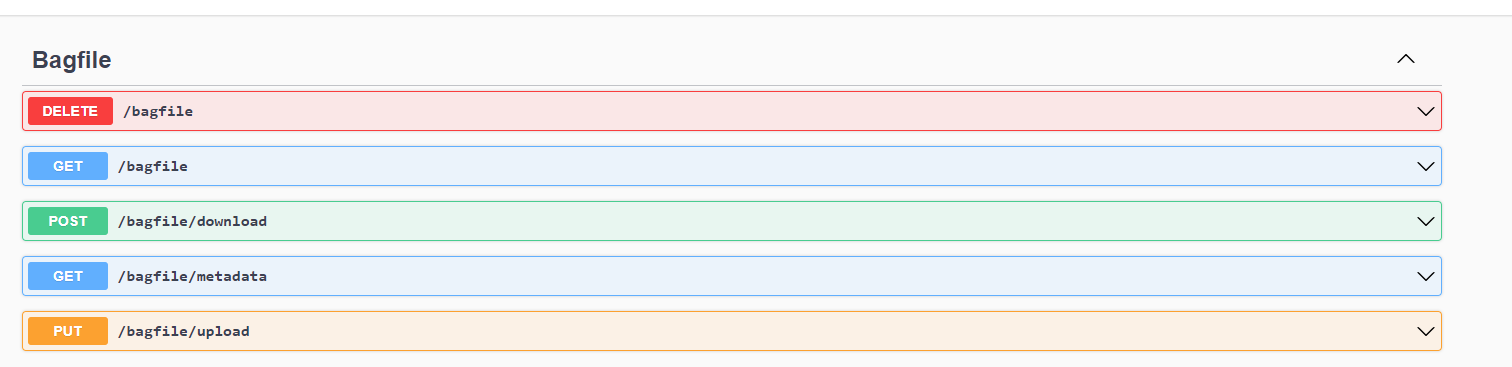
\includegraphics[height=8cm,width=\linewidth]{images/rest-api.png}
		\caption{REST-API endpoints}
	\end{center}
\end{figure}
I tried to implement the above mentioned tasks along with help of my colleagues.
 
Then the communication between the backend and frontend part have been implemted by rossbridge and websockets. Implementation of websockets is just opening of the ports and then waiting for the command to come from frontend. The command from the frontend with comes from the Rosbridge which gives the ROS-API wrapper in json file. I helped in the initial setup of rosbridge and websockets. The small and simple code which is used to test the rosbridge and websockets which is used to communicate between the fronend and backend is shown in below figure.  Then the rest further development of json folder structure is taken care by UI/UX team.
\pagebreak
\begin{figure}[h]
	\begin{center}
		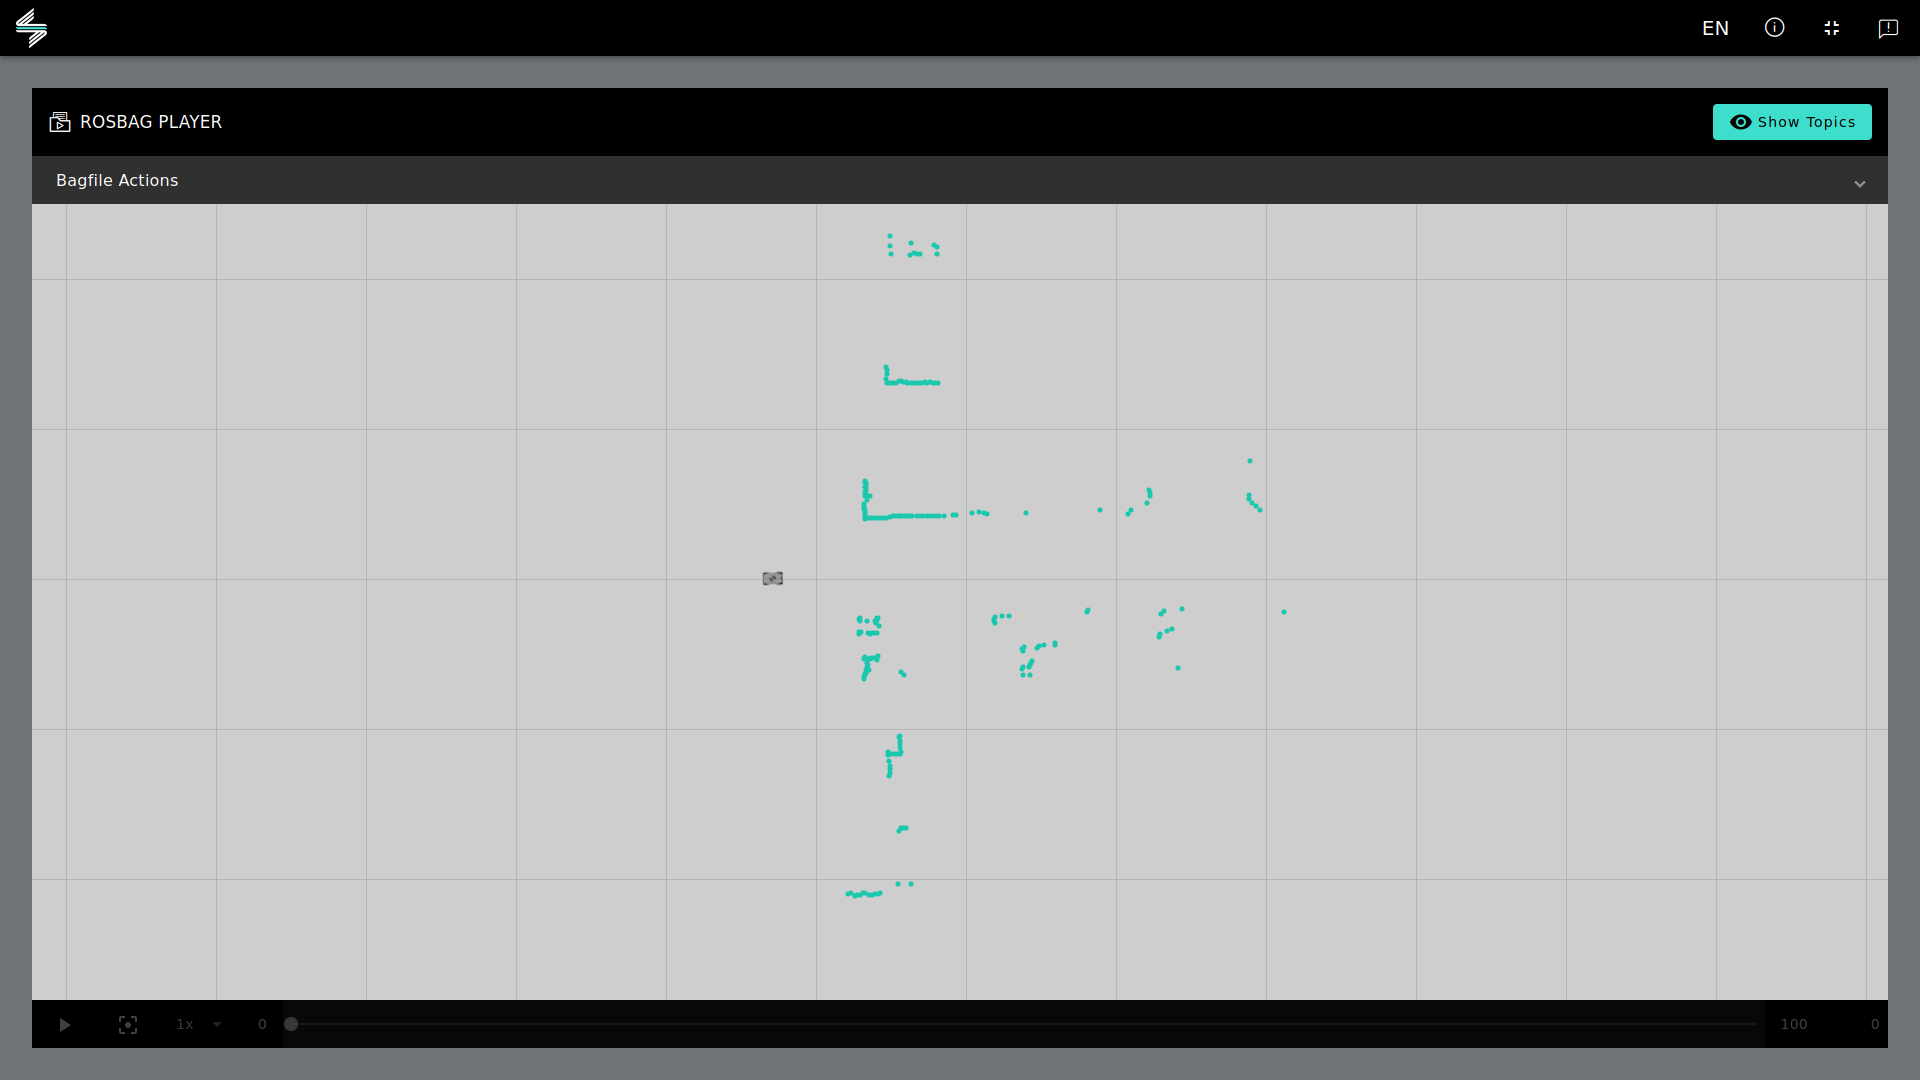
\includegraphics[height=10cm,width=\linewidth]{images/frontend-rosbag.png}
		\caption{Frontend of rosbag player}
	\end{center}
\end{figure}
 
The another task was to make the map visualize in the frontend UI tool. This involved the conversion of occupancy grid to map image. The customer requirement also suggested to find the which version of robot is used based on the file name of the rosbag. This part was implemented by colleagues in the backend team. 

Then the major part of the project, which involved the development of frontend UI for customer. This involved designing the look of the robot, designing of the frontend layouts, subscribing to particular rostopic and analysing and plotting it. All these tasks were done by frontend UI/UX team members.

Currently the functionality of backend is implemented and frontend is able to get some of topics like /odom and all. The buttons for pause/play, slider to jump to particular time, and buttons to change the speed is implemented which will interact with the backend via websockets and rosbridge.The current fronend is as shown in the figure below.